\section{Population vs. Sample}

\begin{definition}
A population is the set of all possible data that meet a specific definition. In the event data from every member of a population can be obtained, we refer to that set of data as the population.
\end{definition}

\begin{definition}
A sample is a subset of a population.  
\end{definition}

\begin{example}
Let the definition for the population be
\begin{center}
    The set of ages for all teachers who work at school A.
\end{center}
Our population is 
\begin{align*}
    G = \{x_{i}: x_{i} \hspace{4pt} \text{is the age for teacher} \hspace{4pt} i \hspace{4pt} \text{who works at school A}\}
\end{align*}
One sample of $G$ could be the set of ages for all science teachers who work at school A
\begin{align*}
    S = \{x_{i}: x_{i} \hspace{4pt} \text{is the age for science teacher} \hspace{4pt} i \hspace{4pt} \text{who works at school A}\}
\end{align*}
Another sample of $G$ could be the set of ages for all chemistry teachers who work at school A
\begin{align*}
    C = \{x_{i}: x_{i} \hspace{4pt} \text{is the age for chemistry teacher} \hspace{4pt} i \hspace{4pt} \text{who works at school A}\}
\end{align*}
\end{example}

\begin{definition}
A parameter is some quantity associated with a population, containing information about a population.
\end{definition}

\begin{definition}
A statistic is some quantity associated with a sample, containing information about a sample. One of the larger goals of an introductory course in statistics is to use, under a set of conditions, a statistic to make statements about the population.  
\end{definition}

\begin{example}
The mean age of all faculty members at school A is a parameter for the population:
\begin{align*}
    G = \{x_{i}: x_{i} \hspace{4pt} \text{is the age for teacher} \hspace{4pt} i \hspace{4pt} \text{who works at school A}\}
\end{align*}
The median age of all science teachers at school A is a statistic for the sample $S$ of $G$:
\begin{align*}
    S = \{x_{i}: x_{i} \hspace{4pt} \text{is the age for science teacher} \hspace{4pt} i \hspace{4pt} \text{who works at school A}\}
\end{align*}
\end{example}

\begin{exercise}
Hospital H contains $225$ patients. The hospital lab contains a pint of blood from $\dfrac{1}{9}^{\text{th}}$ of these patients. Let
\begin{align*}
    B = \{x_{i}: x_{i} \hspace{4pt} \text{is a pint of blood for patient} \hspace{4pt} i \hspace{4pt} \text{in hospital H}\}
\end{align*}
be the set of these pints of blood. Is $B$ a sample or a population? If sample, then describe the population.
\end{exercise}

\begin{exercise}
We have the following sets $D, F,$ and $K$. For each, identify whether it is the population or a sample.
\begin{align*}
    &F = \{x: x \hspace{4pt} \text{is a teacher at school A}\}\\
    &K = \{x: x \hspace{4pt} \text{is a teacher teaching calculus at school A or a student in a calculus course at school A}\}\\
    &D = \{x: x \hspace{4pt} \text{is a student or teacher at school A}\}
\end{align*}
\resizebox{30em}{30em}{%
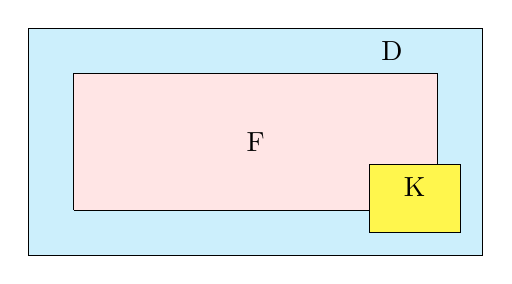
\begin{tikzpicture}[scale=\textwidth/4.2cm]
    % population
    \draw [fill=cyan!20] (0, 0) 
    -- (2, 0)
    -- (2, 1)
    -- (0, 1)
    -- (0, 0);
    \node at (1.6, 0.9) {D};
    % sample 1
    \draw [fill=red!10] (0.2, 0.2) 
    -- (1.8, 0.2)
    -- (1.8, 0.8)
    -- (0.2, 0.8)
    -- (0.2, 0.2);
    \node at (1, 0.5) {F};
    % sample 2
    \draw [fill=yellow!70] (1.5, 0.1)
    -- (1.9, 0.1)
    -- (1.9, 0.4)
    -- (1.5, 0.4)
    -- (1.5, 0.1);
    \node at (1.7, 0.3) {K};
\end{tikzpicture}
}
\end{exercise}

\begin{exercise}
I have contacted $200$ Connecticut state residents within the top, federal income tax bracket and asked them blunt questions about their annual household income. I stored the answers to those questions in a text file on my computer. Did I collect a sample or a population? If sample, what is the population? 
\end{exercise}

\begin{exercise}
The average annual household income for those $200$ Connecticut state residents within the top, federal income tax bracket, whom I most likely vexed with my blunt questioning, is $\$404109$. Is this quantity a parameter or a statistic?
\end{exercise}

\begin{exercise}
I have contacted every member of the Riverside community in Connecticut and asked them blunt questions about their annual household income. Did I collect a sample or a population? If sample, what is the population? 
\end{exercise}